\documentclass[border=8pt]{standalone}
\usepackage{tikz}
\usetikzlibrary{positioning, arrows.meta, shapes.geometric, calc}

% Colors
\definecolor{dim1}{RGB}{86, 163, 239}
\definecolor{dim2}{RGB}{239, 123, 86}
\definecolor{dim3}{RGB}{156, 136, 255}
\definecolor{bg}{RGB}{248, 249, 250}
\definecolor{archbg}{RGB}{243, 243, 243}

\begin{document}
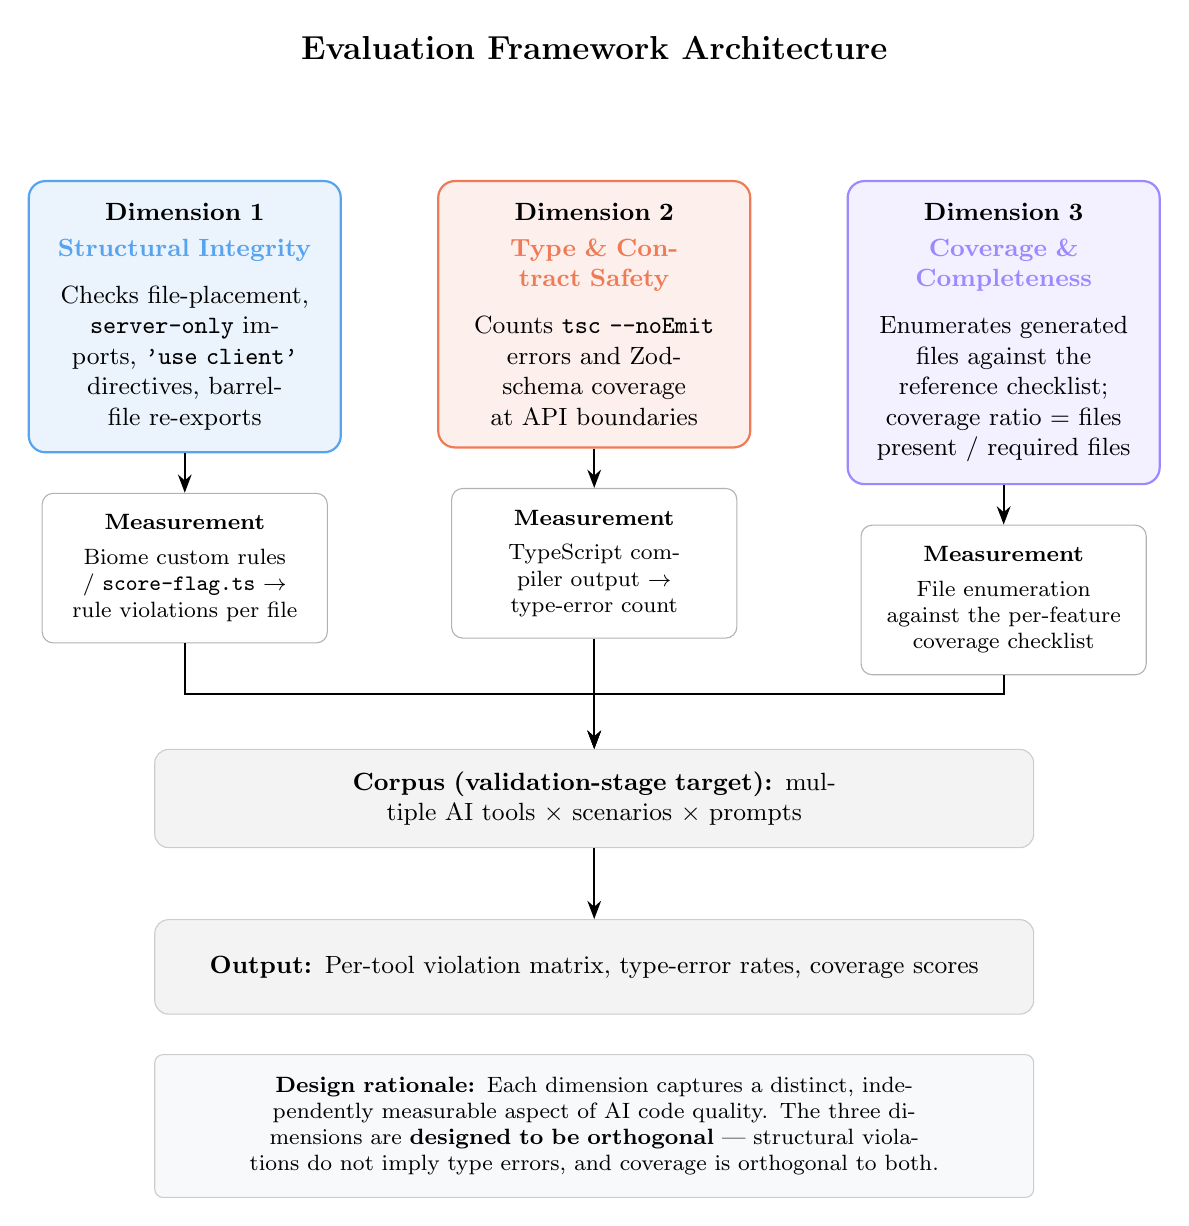
\begin{tikzpicture}[
    node distance=0.9cm and 0.8cm,
    dimbox/.style={draw, rounded corners=6pt, text width=3.4cm, minimum height=2.6cm,
                   align=center, font=\small, inner sep=8pt},
    dim1box/.style={dimbox, fill=dim1!12, draw=dim1, thick},
    dim2box/.style={dimbox, fill=dim2!12, draw=dim2, thick},
    dim3box/.style={dimbox, fill=dim3!12, draw=dim3, thick},
    measure/.style={rectangle, draw=black!30, fill=white, rounded corners=4pt,
                    inner sep=6pt, font=\footnotesize, align=center, text width=3.2cm,
                    minimum height=1.9cm},
    arch/.style={rectangle, draw=black!20, fill=archbg, rounded corners=5pt,
                 inner sep=8pt, font=\small, align=center, text width=10.6cm, minimum height=1.2cm},
    arrow/.style={->, >=Stealth, thick},
]

% Title
\node[font=\large\bfseries] (title) at (0, 0.6) {Evaluation Framework Architecture};

% ============ THREE DIMENSIONS ============
\node[dim1box, below=1.4cm of title, xshift=-5.2cm] (d1) {
    \textbf{Dimension 1}\\[2pt]
    {\color{dim1}\textbf{Structural Integrity}}\\[6pt]
    Checks file-placement, \texttt{server-only} imports, \texttt{'use client'} directives, barrel-file re-exports
};

\node[dim2box, below=1.4cm of title] (d2) {
    \textbf{Dimension 2}\\[2pt]
    {\color{dim2}\textbf{Type \& Contract Safety}}\\[6pt]
    Counts \texttt{tsc --noEmit} errors and Zod-schema coverage at API boundaries
};

\node[dim3box, below=1.4cm of title, xshift=5.2cm] (d3) {
    \textbf{Dimension 3}\\[2pt]
    {\color{dim3}\textbf{Coverage \& Completeness}}\\[6pt]
    Enumerates generated files against the reference checklist; coverage ratio = files present / required files
};

% ============ MEASUREMENT APPROACHES ============
\node[below=0.5cm of d1, measure] (m1) {
    \textbf{Measurement}\\[3pt]
    Biome custom rules / \texttt{score-flag.ts} $\rightarrow$ rule violations per file
};

\node[below=0.5cm of d2, measure] (m2) {
    \textbf{Measurement}\\[3pt]
    TypeScript compiler output $\rightarrow$ type-error count
};

\node[below=0.5cm of d3, measure] (m3) {
    \textbf{Measurement}\\[3pt]
    File enumeration against the per-feature coverage checklist
};

% Arrows from dims to measures
\draw[arrow] (d1) -- (m1);
\draw[arrow] (d2) -- (m2);
\draw[arrow] (d3) -- (m3);

% ============ BOTTOM: CORPUS & OUTPUT ============
\node[arch, below=1.4cm of m2] (corpus) {
    \textbf{Corpus (validation-stage target):} multiple AI tools $\times$ scenarios $\times$ prompts
};

\node[arch, below=0.9cm of corpus] (output) {
    \textbf{Output:} Per-tool violation matrix, type-error rates, coverage scores
};

% Arrows to bottom
\coordinate (joiny) at ($(m2.south)!0.5!(corpus.north)$);
\draw[arrow] (m1.south) |- (joiny) -| (corpus.north);
\draw[arrow] (m2.south) -- (corpus.north);
\draw[arrow] (m3.south) |- (joiny) -| (corpus.north);

\draw[arrow] (corpus) -- (output);

% ============ LEGEND ============
\node[below=0.5cm of output, font=\footnotesize, text width=10.6cm, align=center,
      fill=bg, draw=black!20, rounded corners=3pt, inner sep=8pt] (legend) {
    \textbf{Design rationale:} Each dimension captures a distinct, independently
    measurable aspect of AI code quality. The three dimensions are
    \textbf{designed to be orthogonal} --- structural violations do not imply type errors,
    and coverage is orthogonal to both.
};

\end{tikzpicture}
\end{document}